\documentclass[tikz,border=6pt]{standalone}
\usepackage{tikz}
\usetikzlibrary{arrows.meta,positioning,fit,calc}
\definecolor{ink}{HTML}{222222}
\definecolor{bluefill}{HTML}{E8F1FF}
\definecolor{greenfill}{HTML}{EAF7EF}
\definecolor{amberfill}{HTML}{FFF4D6}
\definecolor{redfill}{HTML}{FDECEC}
\definecolor{grayfill}{HTML}{F3F4F6}
\tikzset{
  box/.style={draw=ink, rounded corners=2pt, very thick, align=center, minimum height=9mm, text width=31mm, font=\sffamily\small},
  smallbox/.style={draw=ink, rounded corners=2pt, thick, align=center, minimum height=8mm, text width=28mm, font=\sffamily\footnotesize},
  arrow/.style={-{Latex[length=2.2mm]}, very thick, draw=ink},
  dasharrow/.style={-{Latex[length=2.2mm]}, thick, dashed, draw=ink}
}
\begin{document}
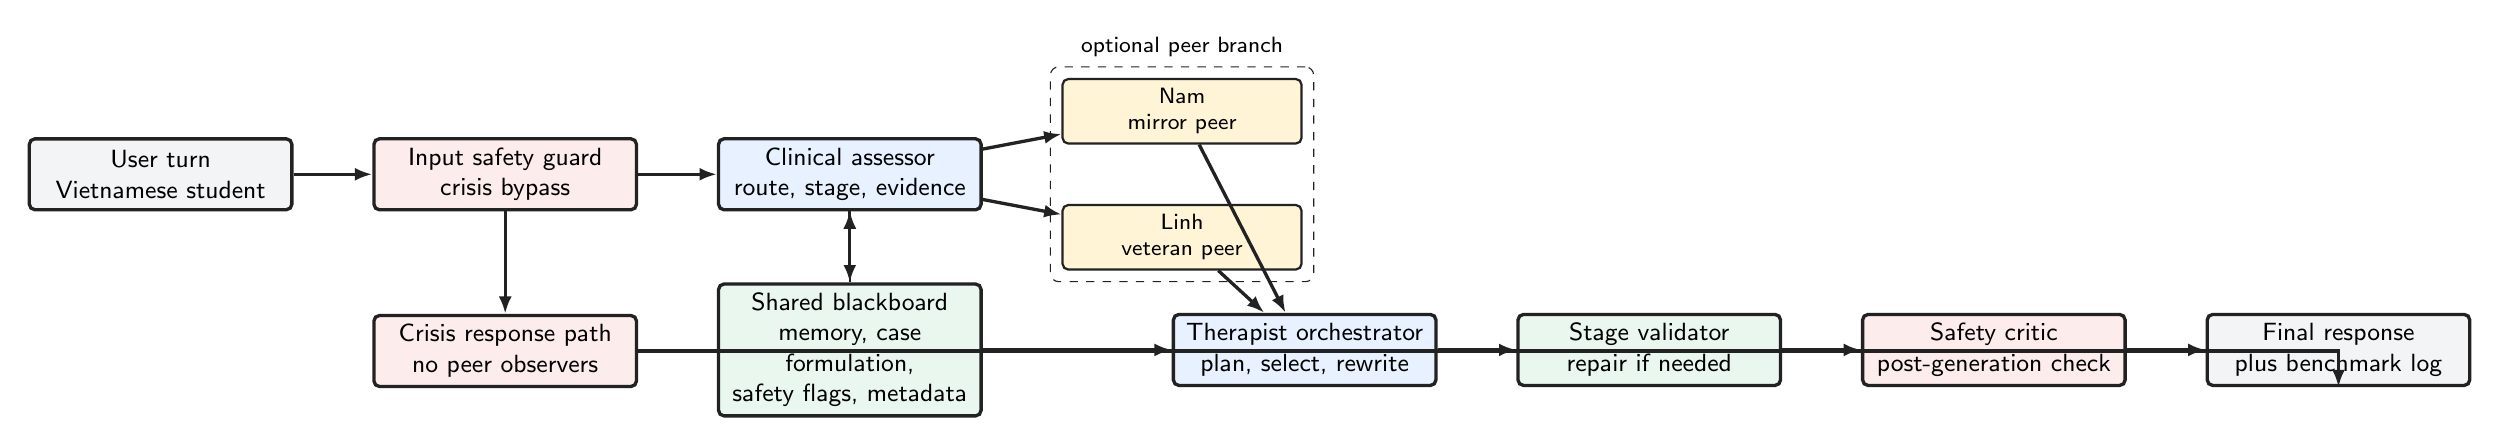
\begin{tikzpicture}[node distance=9mm and 10mm]
  \node[box, fill=grayfill] (user) {User turn\\Vietnamese student};
  \node[box, fill=redfill, right=of user] (safetyin) {Input safety guard\\crisis bypass};
  \node[box, fill=bluefill, right=of safetyin] (assessor) {Clinical assessor\\route, stage, evidence};
  \node[box, fill=greenfill, below=of assessor] (blackboard) {Shared blackboard\\memory, case formulation,\\safety flags, metadata};
  \node[smallbox, fill=amberfill, right=of assessor, yshift=8mm] (nam) {Nam\\mirror peer};
  \node[smallbox, fill=amberfill, right=of assessor, yshift=-8mm] (linh) {Linh\\veteran peer};
  \node[box, fill=bluefill, right=24mm of blackboard] (orch) {Therapist orchestrator\\plan, select, rewrite};
  \node[box, fill=greenfill, right=of orch] (validator) {Stage validator\\repair if needed};
  \node[box, fill=redfill, right=of validator] (critic) {Safety critic\\post-generation check};
  \node[box, fill=grayfill, right=of critic] (out) {Final response\\plus benchmark log};
  \node[box, fill=redfill, below=13mm of safetyin] (crisis) {Crisis response path\\no peer observers};

  \draw[arrow] (user) -- (safetyin);
  \draw[arrow] (safetyin) -- (assessor);
  \draw[arrow] (safetyin) -- (crisis);
  \draw[arrow] (assessor) -- (blackboard);
  \draw[dasharrow] (blackboard) -- (assessor);
  \draw[arrow] (assessor) -- (nam);
  \draw[arrow] (assessor) -- (linh);
  \draw[arrow] (nam) -- (orch);
  \draw[arrow] (linh) -- (orch);
  \draw[arrow] (blackboard) -- (orch);
  \draw[arrow] (orch) -- (validator);
  \draw[arrow] (validator) -- (critic);
  \draw[arrow] (critic) -- (out);
  \draw[arrow] (crisis.east) -| (out.south);

  \node[draw=ink, rounded corners=3pt, dashed, fit=(nam)(linh), inner sep=4pt, label={[font=\sffamily\footnotesize]above:optional peer branch}] {};
\end{tikzpicture}
\end{document}
